\let\negmedspace\undefined
\let\negthickspace\undefined
\documentclass[journal]{IEEEtran}
\usepackage{caption}
\usepackage[a5paper, margin=10mm, onecolumn]{geometry}
%\usepackage{lmodern} % Ensure lmodern is loaded for pdflatex
\usepackage{tfrupee} % Include tfrupee package

\setlength{\headheight}{1cm} % Set the height of the header box
\setlength{\headsep}{0mm}     % Set the distance between the header box and the top of the text

\usepackage{gvv-book}
\usepackage{gvv}
\usepackage{cite}
\usepackage{amsmath,amssymb,amsfonts,amsthm}
\usepackage{algorithmic}
\usepackage{graphicx}
\usepackage{textcomp}
\usepackage{xcolor}
\usepackage{txfonts}
\usepackage{listings}
\usepackage{enumitem}
\usepackage{mathtools}
\usepackage{gensymb}
\usepackage{comment}
\usepackage[breaklinks=true]{hyperref}
\usepackage{tkz-euclide} 
\usepackage{listings}
% \usepackage{gvv}                                        
\def\inputGnumericTable{}                                 
\usepackage[latin1]{inputenc}                                
\usepackage{color}                                            
\usepackage{array}                                            
\usepackage{longtable}                                       
\usepackage{calc}                                             
\usepackage{multirow}                                         
\usepackage{hhline}                                           
\usepackage{ifthen}                                           
\usepackage{lscape}
\begin{document}

\bibliographystyle{IEEEtran}


\title{1.5.10}
\author{EE25BTECH11022 - sankeerthan}
% \maketitle
% \newpage
% \bigskip
{\let\newpage\relax\maketitle}

\renewcommand{\thefigure}{\theenumi}
\renewcommand{\thetable}{\theenumi}
\setlength{\intextsep}{10pt} % Space between text and floats


\numberwithin{equation}{enumi}
\numberwithin{figure}{enumi}
\renewcommand{\thetable}{\theenumi}


\textbf{problem(1.5.10)}.
Find the ratio in which the line segment joining the points 
$\vec{A}\brak{5, -6}$ and $\vec{B}\brak{-1, -4}$ is divided by X-axis. Also,find the coordinates of the  point of division

\textbf{Solution}:

Let the given points be A and B
\begin{align*} \vec{A} = \myvec{1 \\ -5}, \vec{B} = \myvec{-4 \\ 5} \end{align*}
Let the X-axis divide the line segment \(\overline{\vec{AB}}\) at point $\vec{P}$ in the ratio $k:1$.
Since $\vec{P}$ lies on X-axis, let
\begin{align*}
\vec{P} = \myvec{x \\ 0}
\end{align*}
The point $\vec{A}$, $\vec{B}$, $\vec{P}$ are collinear.
\begin{align}
\implies \text{rank}\myvec{\vec{B}-\vec{A} & \vec{P}-\vec{A}} = 1
\end{align}
\begin{align}
\myvec{-5 & x-1 \\ 10 & 5} \xleftrightarrow{R_1 \rightarrow {R_1 + \frac{1}{2}R_2}}\myvec{0 & x-\frac{3}{2} \\ 10 & 5} \xleftrightarrow{R_1 \leftrightarrow R_2}  \myvec{10 & 5 \\ 0 & x-\frac{3}{2}}
\end{align}
The number of nonzero rows in the row reduced matrix (also known as {\em echelon form}) is defined as the rank. For above matrix to be of rank 1,
\begin{align}
x+\frac{3}{2} &= 0 \\
x &= \frac{-3}{2}
\end{align}
$\therefore$ The coordinates of the point of intersection are 
\begin{align*}
\vec{P} = \myvec{\frac{-3}{2} \\ 0}
\end{align*}

Substituting the values of $\vec{A}$, $\vec{B}$ and $\vec{P}$,
\begin{align}
k=\frac{\myvec{\frac{5}{2} & -5}\myvec{\frac{5}{2} \\ -5}}{\norm{\myvec{\frac{5}{2} \\ -5}}^2}=1
\end{align}

Thus, the ratio in which the point $\vec{P}$ divides the line segment $\vec{AB}$ is \textbf{1:1}. 

\begin{figure}
   \centering
   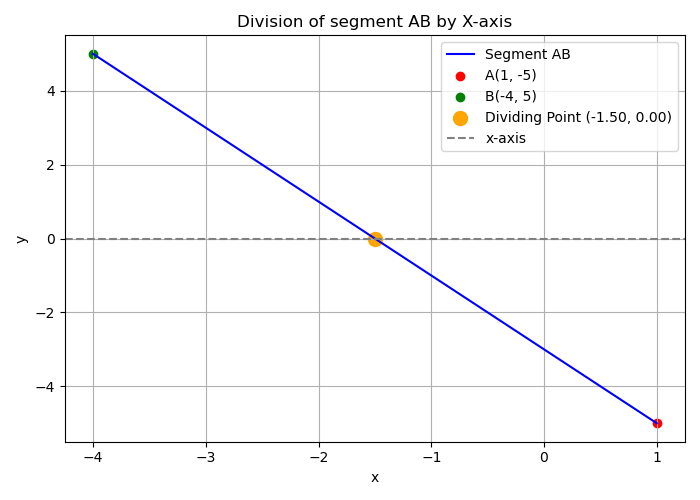
\includegraphics[width=1\columnwidth]{figs/points.png}
   \caption{Plot of line segment \textbf{AB}}
   \label{}
\end{figure}

\end{document}
